%%%%%%%%%%%%%%%%%%%%%%%%%%%%%%%%%%%%%%%%%
% NIWeek 2014 Poster by T. Reveyrand
% www.microwave.fr
% http://www.microwave.fr/LaTeX.html
% ---------------------------------------
% 
% Original template created by:
% Brian Amberg (baposter@brian-amberg.de)
%
% This template has been downloaded from:
% http://www.LaTeXTemplates.com
%
% License:
% CC BY-NC-SA 3.0 (http://creativecommons.org/licenses/by-nc-sa/3.0/)
%
%%%%%%%%%%%%%%%%%%%%%%%%%%%%%%%%%%%%%%%%%

%----------------------------------------------------------------------------------------
%	PACKAGES AND OTHER DOCUMENT CONFIGURATIONS
%----------------------------------------------------------------------------------------

\documentclass[ansiepaperDNP,portrait]{baposter}

\usepackage[font=small,labelfont=bf]{caption} % Required for specifying captions to tables and figures
\usepackage{booktabs} % Horizontal rules in tables
\usepackage{relsize} % Used for making text smaller in some places

\usepackage{amsmath,amsfonts,amssymb,amsthm} % Math packages
\usepackage{eqparbox}

\usepackage{textcomp}
\usepackage{multicol}
\usepackage{wrapfig} % Allows wrapping text around tables and figures

\graphicspath{{figures/}} % Directory in which figures are stored

 %\definecolor{bordercol}{RGB}{40,40,40} % Border color of content boxes
 \definecolor{bordercol}{RGB}{211,211,211} % Border color of content boxes

 \definecolor{headercol1}{RGB}{0,102,51} % Background color for the header in the content boxes (left side)
\definecolor{headercol2}{RGB}{0,102,51} 
% \definecolor{headercol2}{RGB}{120,120,120} % Background color for the header in the content boxes (right side)
 \definecolor{headerfontcol}{RGB}{256,256,256} % Text color for the header text in the content boxes
 %\definecolor{boxcolor}{RGB}{210,235,250} % Background color for the content in the content boxes
\definecolor{boxcolor}{RGB}{250,250,250}

\renewcommand\refname{\vskip -1.35cm}

\begin{document}
\background{}

\begin{poster}{
grid=false,
borderColor=bordercol, % Border color of content boxes
headerColorOne=headercol1, % Background color for the header in the content boxes (left side)
headerColorTwo=headercol2, % Background color for the header in the content boxes (right side)
headerFontColor=headerfontcol, % Text color for the header text in the content boxes
boxColorOne=boxcolor, % Background color for the content in the content boxes
headershape=roundedright, % Specify the rounded corner in the content box headers
headerfont=\Large\sf\bf, % Font modifiers for the text in the content box headers
textborder=rectangle,
background=user,
headerborder=open, % Change to closed for a line under the content box headers
boxshade=plain
}
{
\includegraphics[scale=0.10]{logo_davidson.png}}
%
%----------------------------------------------------------------------------------------
%	TITLE AND AUTHOR NAME
%----------------------------------------------------------------------------------------
%
{ \bf  \huge {A Streamlined Python Framework for AT-TPC Data Analysis} }
%\Large \it A} % Poster title
{\vspace{0.3em} \smaller J.Z. Taylor$^1$, J. Bradt$^2$, D. Bazin$^2$, M.P. Kuchera$^1$ \\  % Authors
  
\smaller $^1$\it{Department of Physics, Davidson College} \\
	     $^2$\it{National Superconducting Cyclotron Laboratory, Michigan State University}}
	    {
\includegraphics[scale=0.3]{nscl_logo.png}} % University/lab logo

%----------------------------------------------------------------------------------------
%	ABSTRACT
%----------------------------------------------------------------------------------------
\headerbox{Abstract}{name=abstract,column=0,row=0, span=3}{
\small{User-friendly data analysis software has been developed for the Active-Target Time Projection Chamber (AT-TPC) experiment at the National Superconducting Cyclotron Laboratory at Michigan State University. The AT-TPC, commissioned in 2014, is a gas-filled detector that acts as both the detector and target for high-efficiency detection of low-intensity, exotic nuclear reactions. The pytpc framework is a Python package for analyzing AT-TPC data. The package was developed for the analysis of $^{46}$Ar(p, p) data. The existing software was used to analyze data produced by the $^{40}$Ar(p, p) experiment that ran in August, 2015. Usage of the package was documented in an analysis manual both to improve analysis steps and aid in the work of future AT-TPC users. Software features and analysis methods in the pytpc framework will be presented along with the $^{40}$Ar results.}
}
%----------------------------------------------------------------------------------------
%	THE AT-TPC
%----------------------------------------------------------------------------------------
\headerbox{The Active-Target Time Projection Chamber}{name=attpc,column=1,row=1,span=2,below=abstract}
{\small{The AT-TPC is a gas-filled detector that acts as both the detector and target for high-efficiency detection of low-intensity, exotic nuclear reactions. Because the gas target also acts as the detector, the AT-TPC is highly efficient, providing nearly ${4\pi}$ angular coverage. The AT-TPC operates inside a nearly 2 Tesla solenoidal magnetic field. Reactions can be measured over a wide range of energies as the beam loses energy in the gas \cite{ATTPC-NIM}.
In order to obtain this ${4\pi}$ coverage with high resolution, a highly segmented pad plane captures the detector signal. There are 10240 pads in the pad plane which produces on the order of 10MB raw of data per event.}

\begin{center}
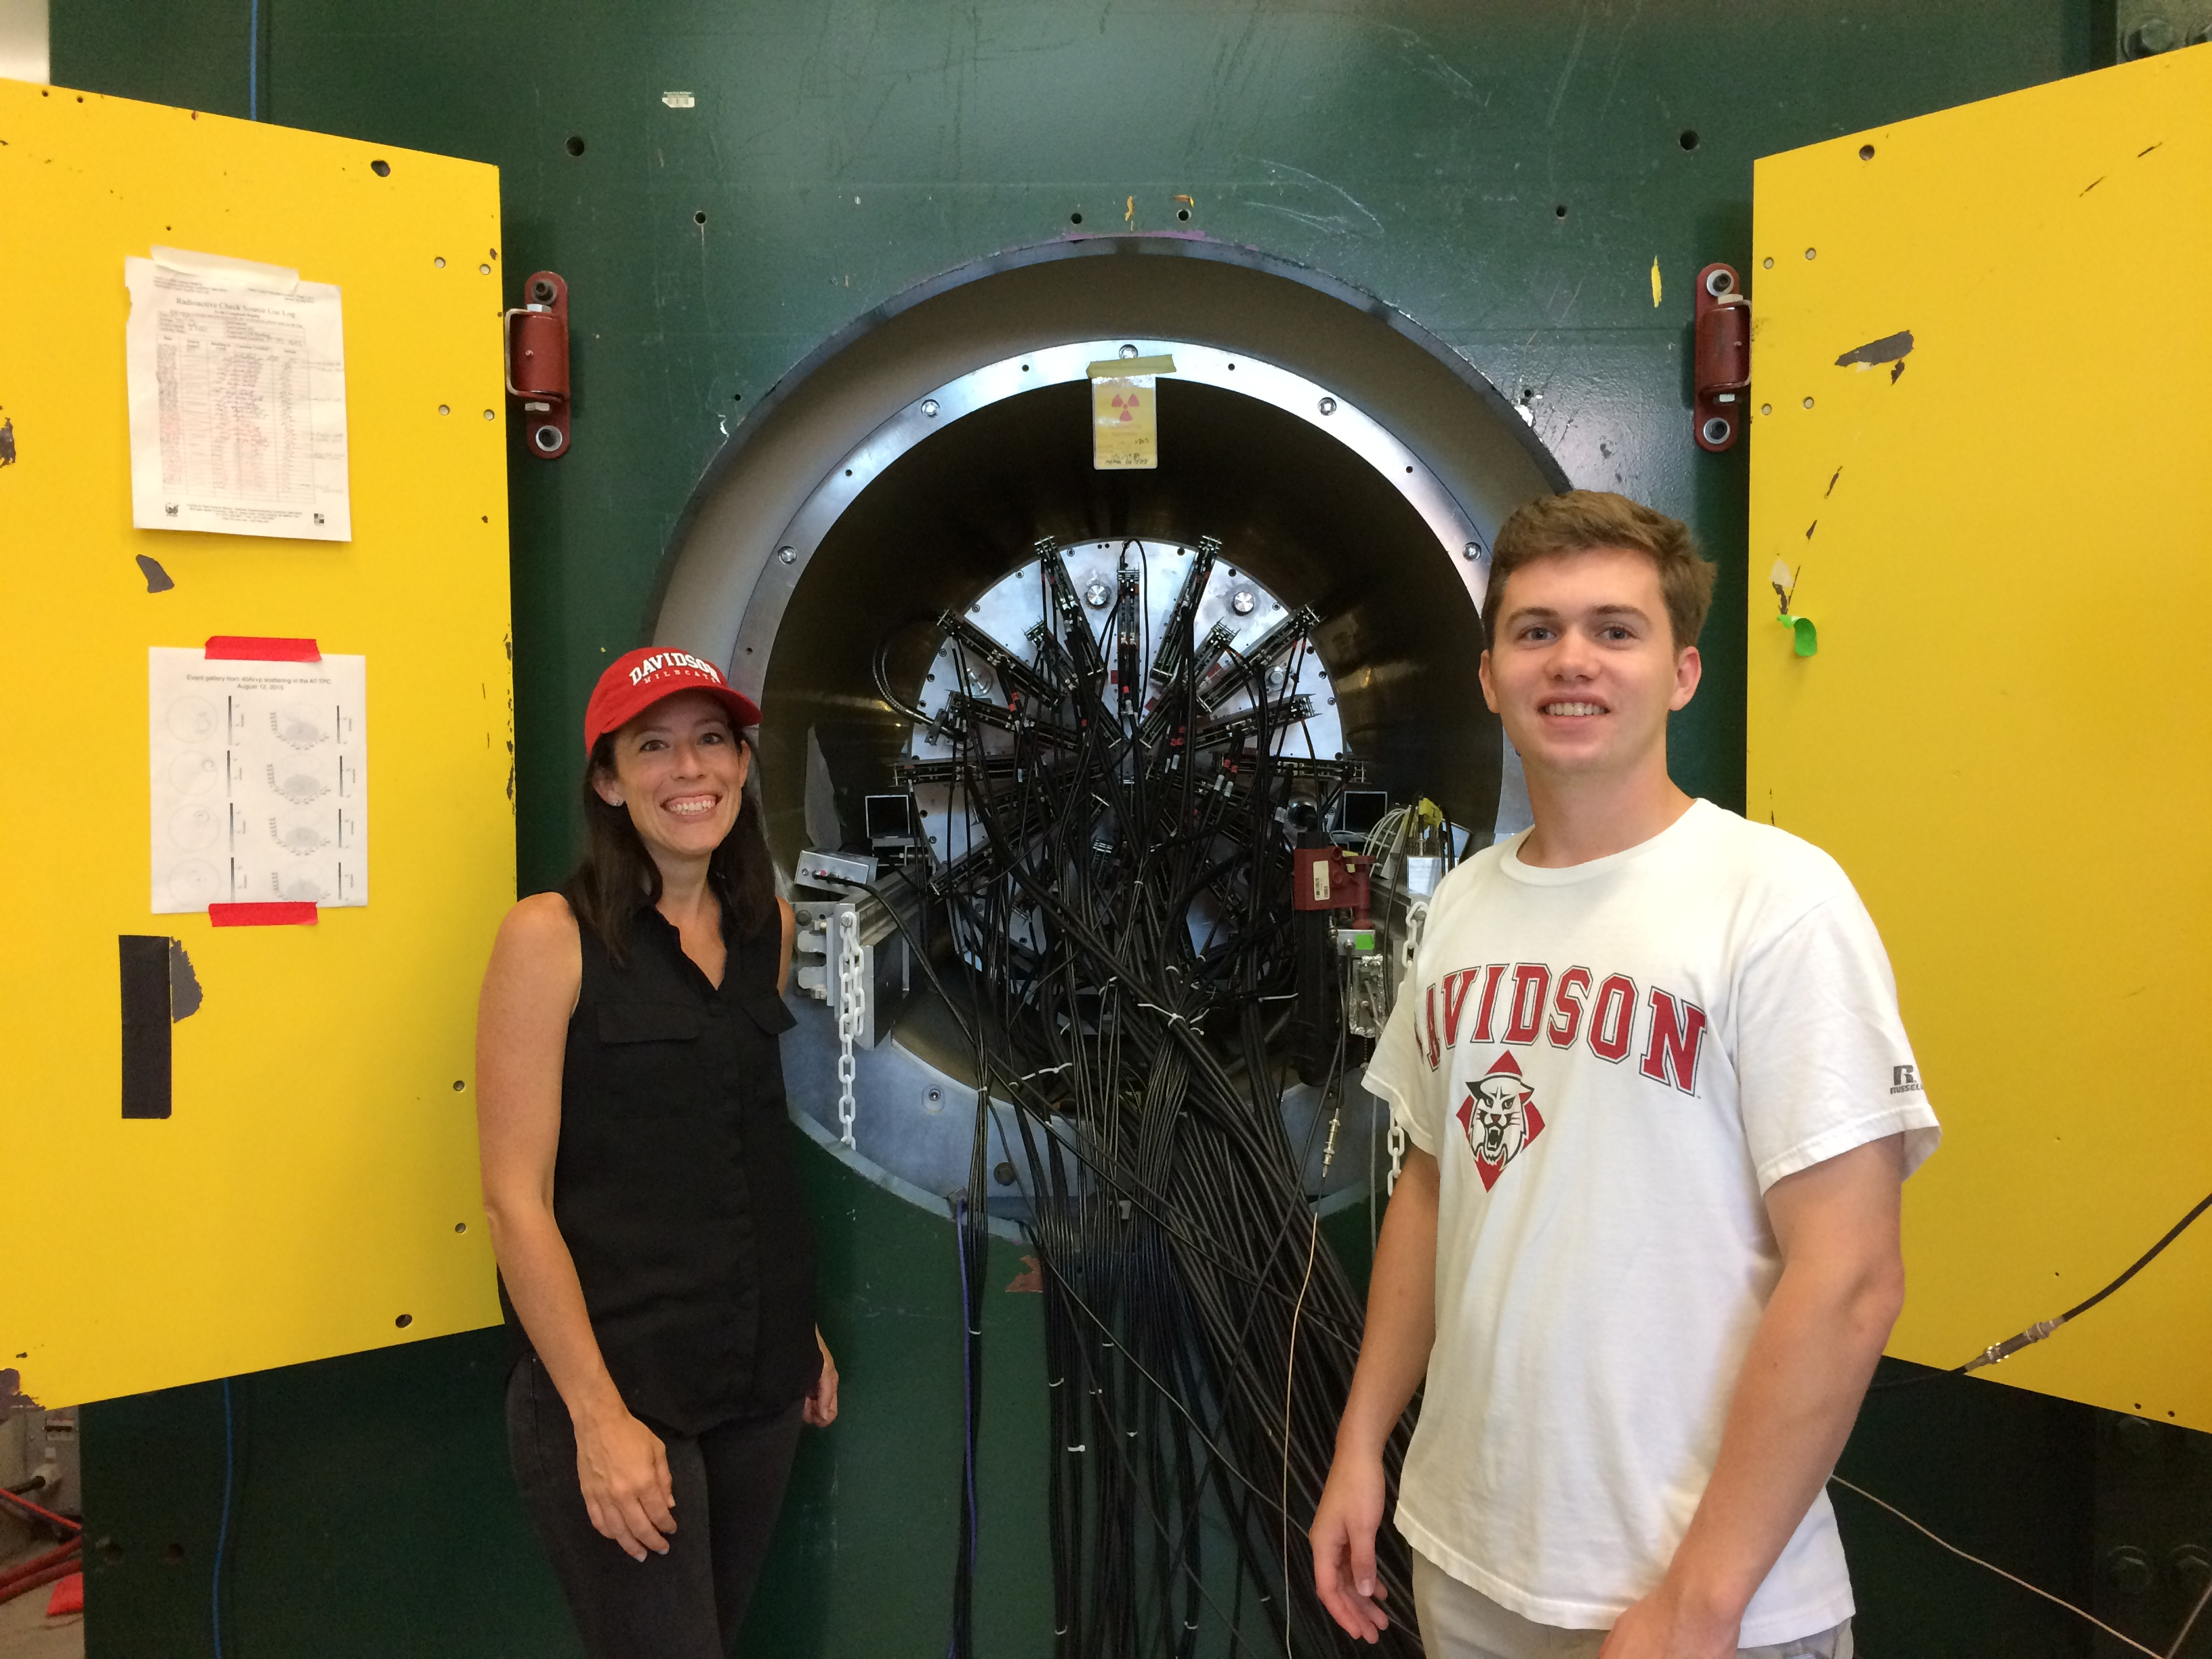
\includegraphics [height=30mm]{michigan_trip.jpg} 
\hspace{0.2cm}
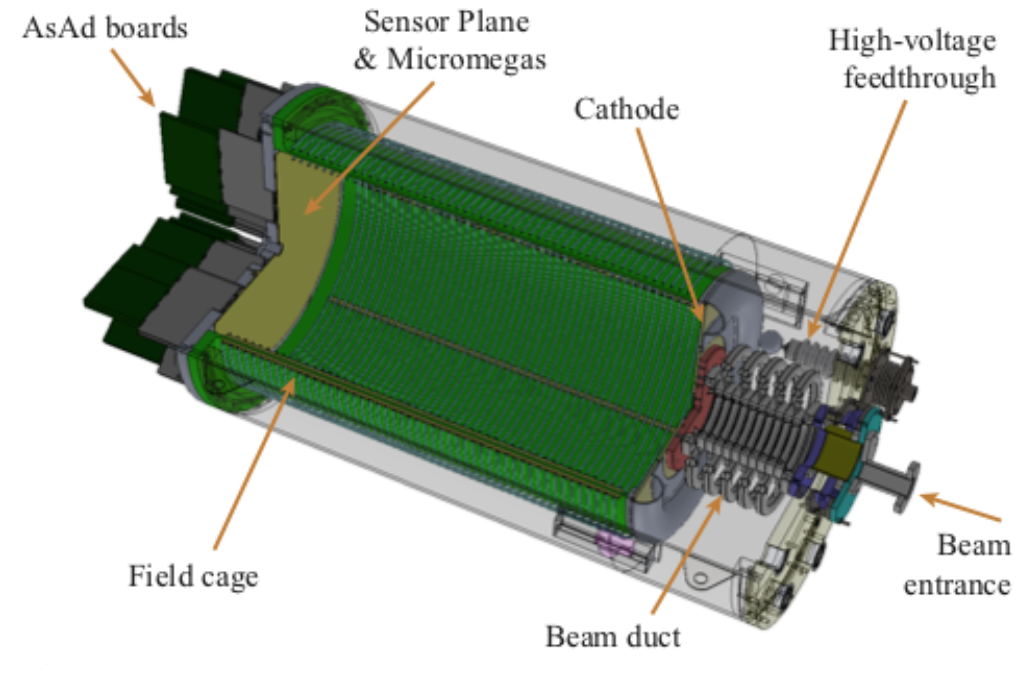
\includegraphics [height=30mm] {attpc.png}
\hspace{0.2cm}
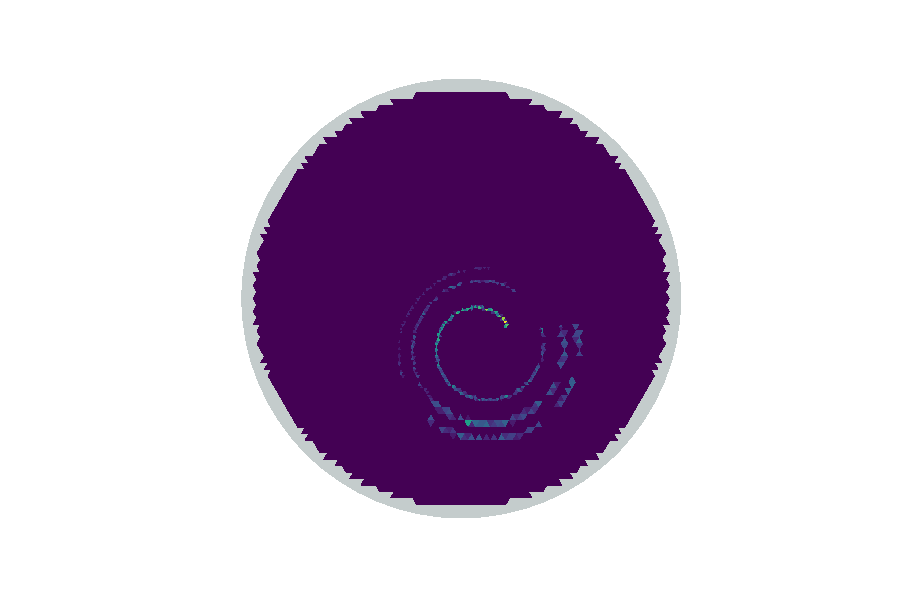
\includegraphics [height=30mm] {padplane.pdf}
\end{center}


\small{\textbf{Fig 2.} Left, a photograph of the pad plane end of the AT-TPC, shown mounted in the solenoid magnet.}

\small{\textbf{Fig 3.} Center, a schematic of the AT-TPC with the outer shielding made transparent. The rare isotope beam enters the the detector on the right-hand side and moves left towards the pad plane \cite{Bradt-thesis}.}

\small{\textbf{Fig 4.} Right, PAD PLANE a plot of the pad plane resolution with a segmented proton event.}

}
%----------------------------------------------------------------------------------------
%	Motivation
%----------------------------------------------------------------------------------------
\headerbox{Motivation}
{name=motivation,column=0,row=1,span=1, below=abstract}
{\small{We study rare isotopes to expand our understanding of the shell structure of nuclei. The AT-TPC was designed and built for improved data acquisition in rare isotope experiments. Rare isotope beams typically have low intensity, leading to fewer reactions and events, thus requiring a detector with high efficiency. In the AT-TPC, the gas that fills the chamber acts both the detector and target, making the detector highly efficient and allowing measurement of reactions occurring at many energies. We are interested in studying the structure of unbound states of isotopes and do so by calculating excitation functions or differential cross sections. The wide energy variance of the data collected in the AT-TPC enables us to calculate excitation functions for a large range of energies.

This project involved creating an analysis manual and framework documentation to streamline the analysis process for users and increase the accessibility of the software as well as analyzing data from the $^{40}$Ar(p,p) reaction.}

\begin{center}
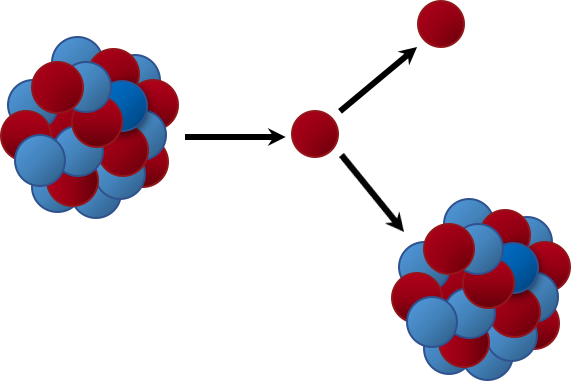
\includegraphics[width=40mm]{ar40_p.png}
\end{center}

\small{\textbf{Fig. 1.} Elastic proton scattering of a $^{40}$Ar nucleus.}
}
%----------------------------------------------------------------------------------------
%	40AR ANALYSIS
%----------------------------------------------------------------------------------------
\headerbox{Analysis of the $^{40}$Ar Beam Experiment Data}{name=analysis,span=2,column=1,row=1, below=attpc}
{\small{The analysis code, originally written for a $^{46}$Ar data, was applied to data from the $^{40}$Ar(p, p) experiment that ran at the NSCL in August,  2015.}
\small{The Monte Carlo fit results provide the vertex position of a reaction in the detector chamber. The energy of the beam particle at this location can be found by calculating the energy lost by the particle to the gas target that fills the chamber.}

\begin{center}
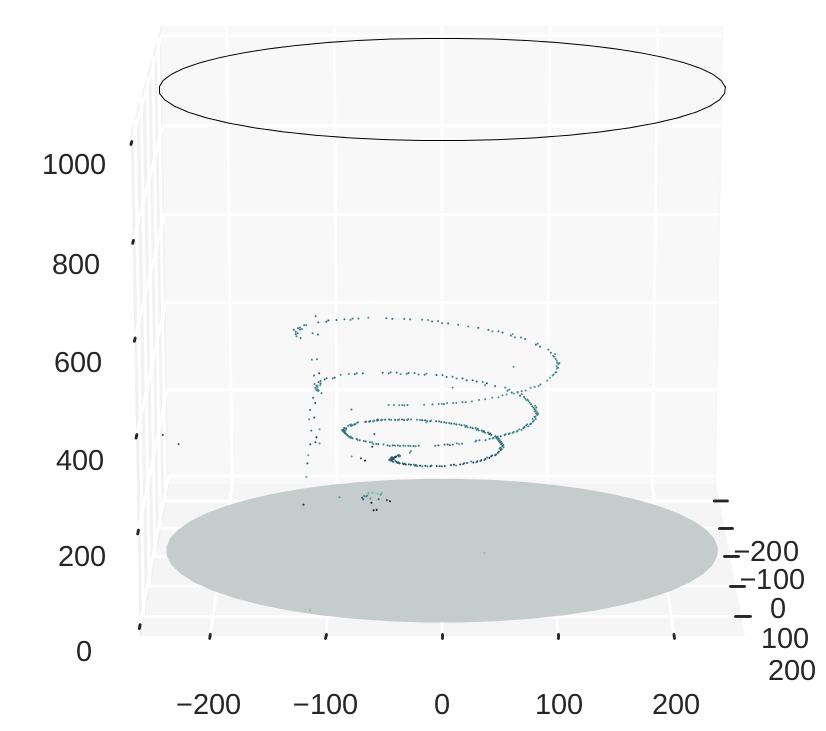
\includegraphics[height=30mm]{chamber_plot.png}
\hspace{.75cm}
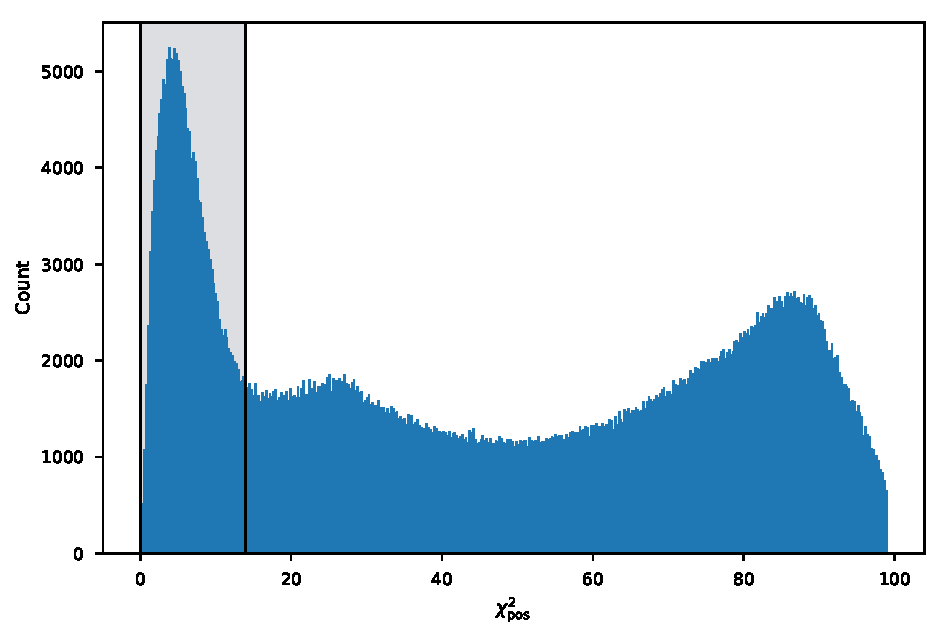
\includegraphics [height=30mm] {chi2pos.pdf}
%\hspace{.75cm}
%\includegraphics [height=30mm] {}
\end{center}

\small{\textbf{Fig 5.} Left, an example of a proton event rendered in the pytpc framework.}

\small{\textbf{Fig 6.} Center, the distribution of $\chi_{pos}^{2}$ values. Events falling above the threshold of 14 were discarded.}

\small{\textbf{Fig 7.} Right, NEW FIGURE}

\begin{center}
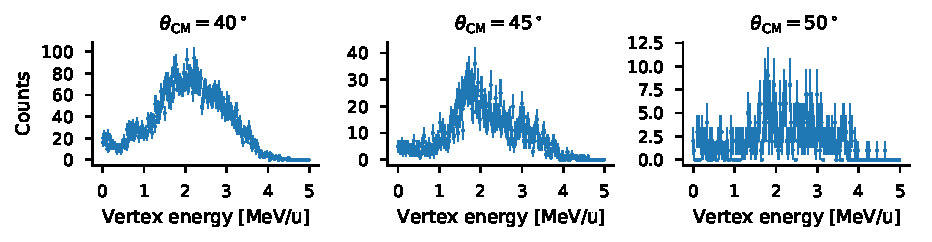
\includegraphics [width=95mm] {angular_excitation_hists_POSTER.pdf}
\end{center}
\small{\textbf{Fig 8.} Unnormalized excitation functions as a function of the $^{40}$Ar vertex energy in the laboratory frame shown for multiple center-of-mass scattering angles ($\theta_{cm}$).}
}

%----------------------------------------------------------------------------------------
%	ACKNOWLEDGEMENTS
%----------------------------------------------------------------------------------------
\headerbox{Acknowledgements}{name=acknowledgements,column=1,above=bottom,span=2}
{\small{This work was supported by NSF grant no. 10049216.\\ Conference funds were supported by the Society of Physics Students.
}


\includegraphics[height=15mm]{nsf_logo.png}
\hspace{.75cm}

\includegraphics [height=15mm]{sps_logo.png}


}
%----------------------------------------------------------------------------------------
%	CONCLUSION - FUTURE
%----------------------------------------------------------------------------------------
\headerbox{Conclusion and Future Work}{name=conclusion,column=1,below=analysis, above=acknowledgements,span=2}
{\small{By analyzing the data from the $^{40}$Ar experiment I tested the adaptability of the software and examined previously unanalyzed experimental data. The analysis manual for the pytpc framework is now being used by the AT-TPC's many external users.

Currently, I am applying machine learning methods to the issue of event classification for AT-TPC data. Ideally, this will increase statistics and reduce both error and computational time.}
}

%----------------------------------------------------------------------------------------
%	REFERENCES
%----------------------------------------------------------------------------------------
\headerbox{References}{name=references,column=0,above=bottom,span=1}{
\footnotesize{\bibliographystyle{unsrt}
\hspace{-2.00cm}
%\itemsep-0.5em
\bibliography{bibliographyDNP.bib}}
}
%----------------------------------------------------------------------------------------
%	PYTPC
%----------------------------------------------------------------------------------------
\headerbox{The pytpc Framework}{name=pytpc,column=0,row=2, above=references, below=motivation}
{\small{The pytpc framework is a Python package for analyzing AT-TPC data. The package provides functions for reconstructing, cleaning, and fitting particle tracks produced in the AT-TPC. Analysis of AT-TPC data is a multi-step process:

\begin{enumerate}\itemsep-0.04em
\item Baseline Correction for Electronics Signals
\item Track Reconstruction
\item Noise Removal
\item Modeling and Fitting Tracks with a Monte Carlo Optimizer
\end{enumerate}

\begin{center}
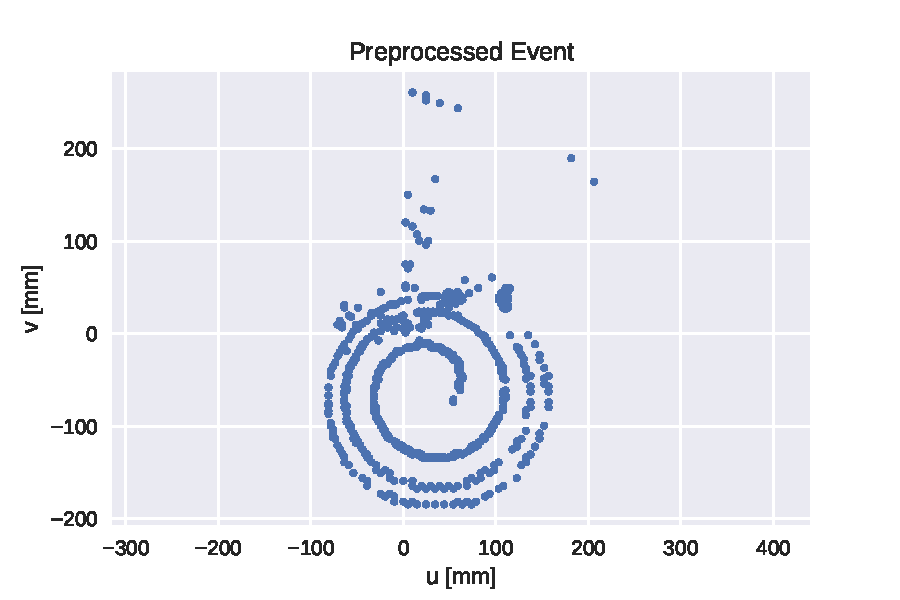
\includegraphics [width=30mm] {preprocess_evt.pdf}
\hspace{0cm}
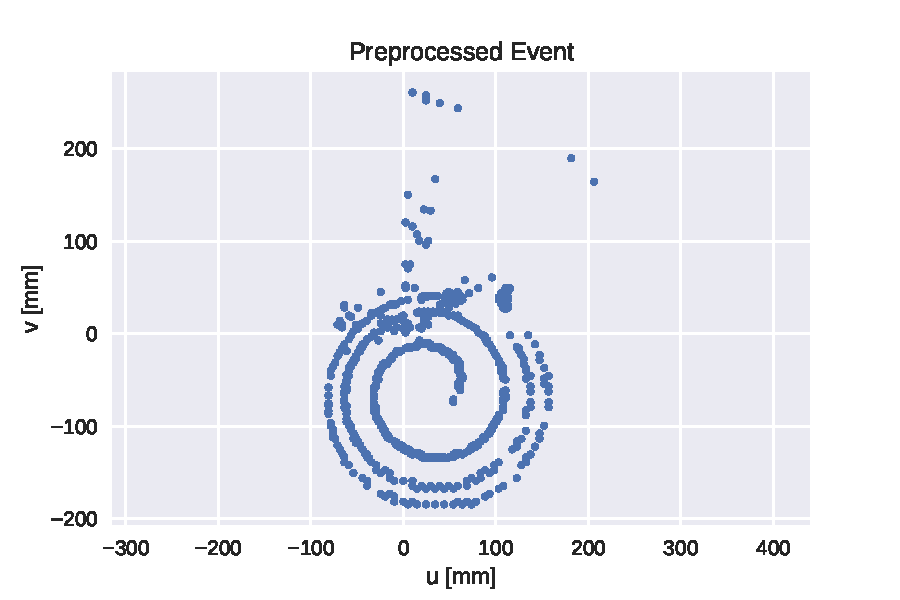
\includegraphics [width=30mm] {preprocess_evt.pdf}
\hspace{3cm}
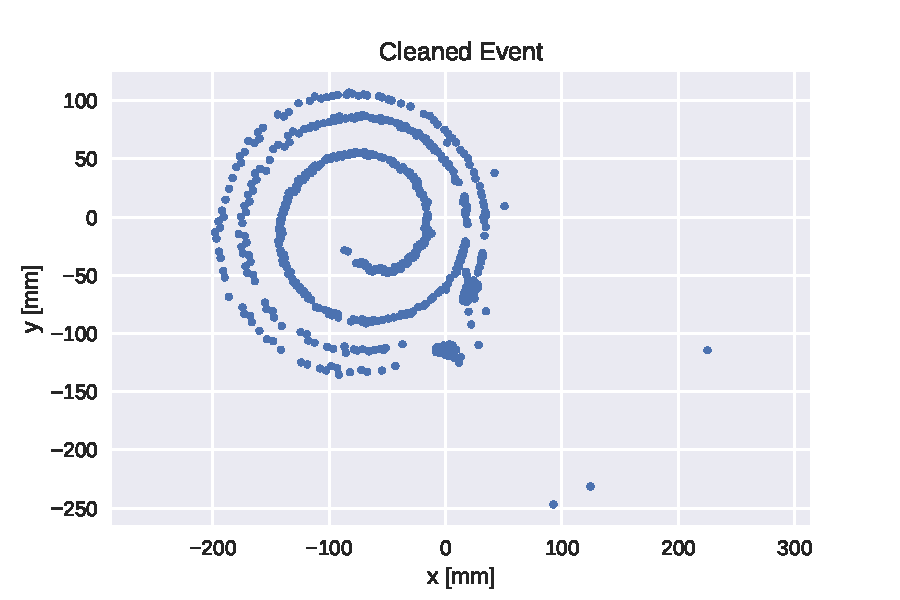
\includegraphics [width=30mm] {clean_evt.pdf}
\hspace{0cm}
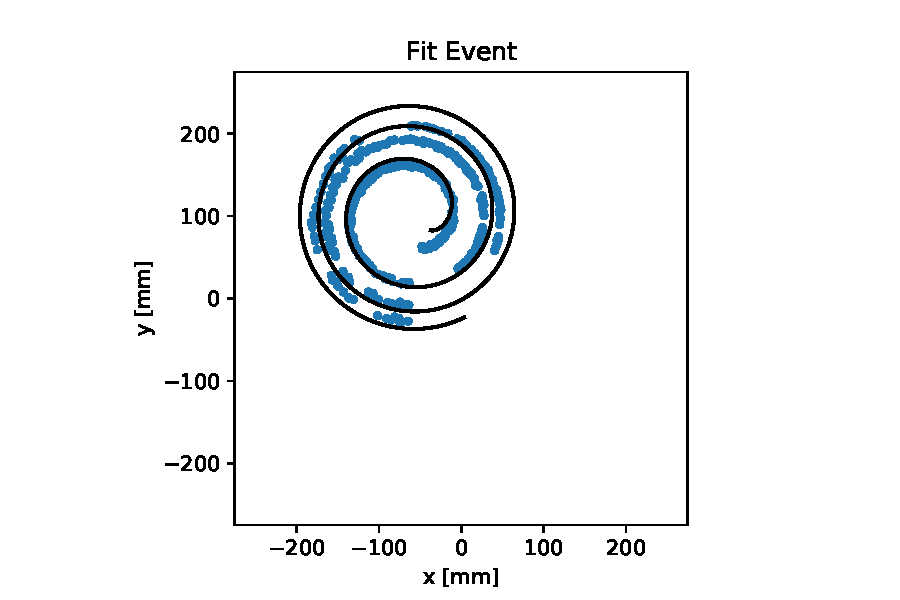
\includegraphics [width=30mm] {fit_evt.pdf}
\end{center}
\textbf{Fig 4.} A preprocessed event (top), an event after the Hough Transform cleaning (bottom left), and a Monte Carlo fit event (bottom right).}
} 

\end{poster}
\end{document}
